\chapter{WKB近似}
这一整章涉及到的内容特别针对于\textbf{一维薛定谔定态方程}的近似求解问题,其实是一种半经典近似,最终我们要得到历史上有名的Sommerfeld量子化条件。

经典力学里面粒子的运动区域是$E>V(x)$,而量子力学允许隧穿,所以我们还要考虑$E<V(x)$的区域,最后我们会去考虑$E\approx V(x)$的区域如何近似。

\section{基本原理}
\subsection*{经典区域}
\begin{figure}
	\centering
	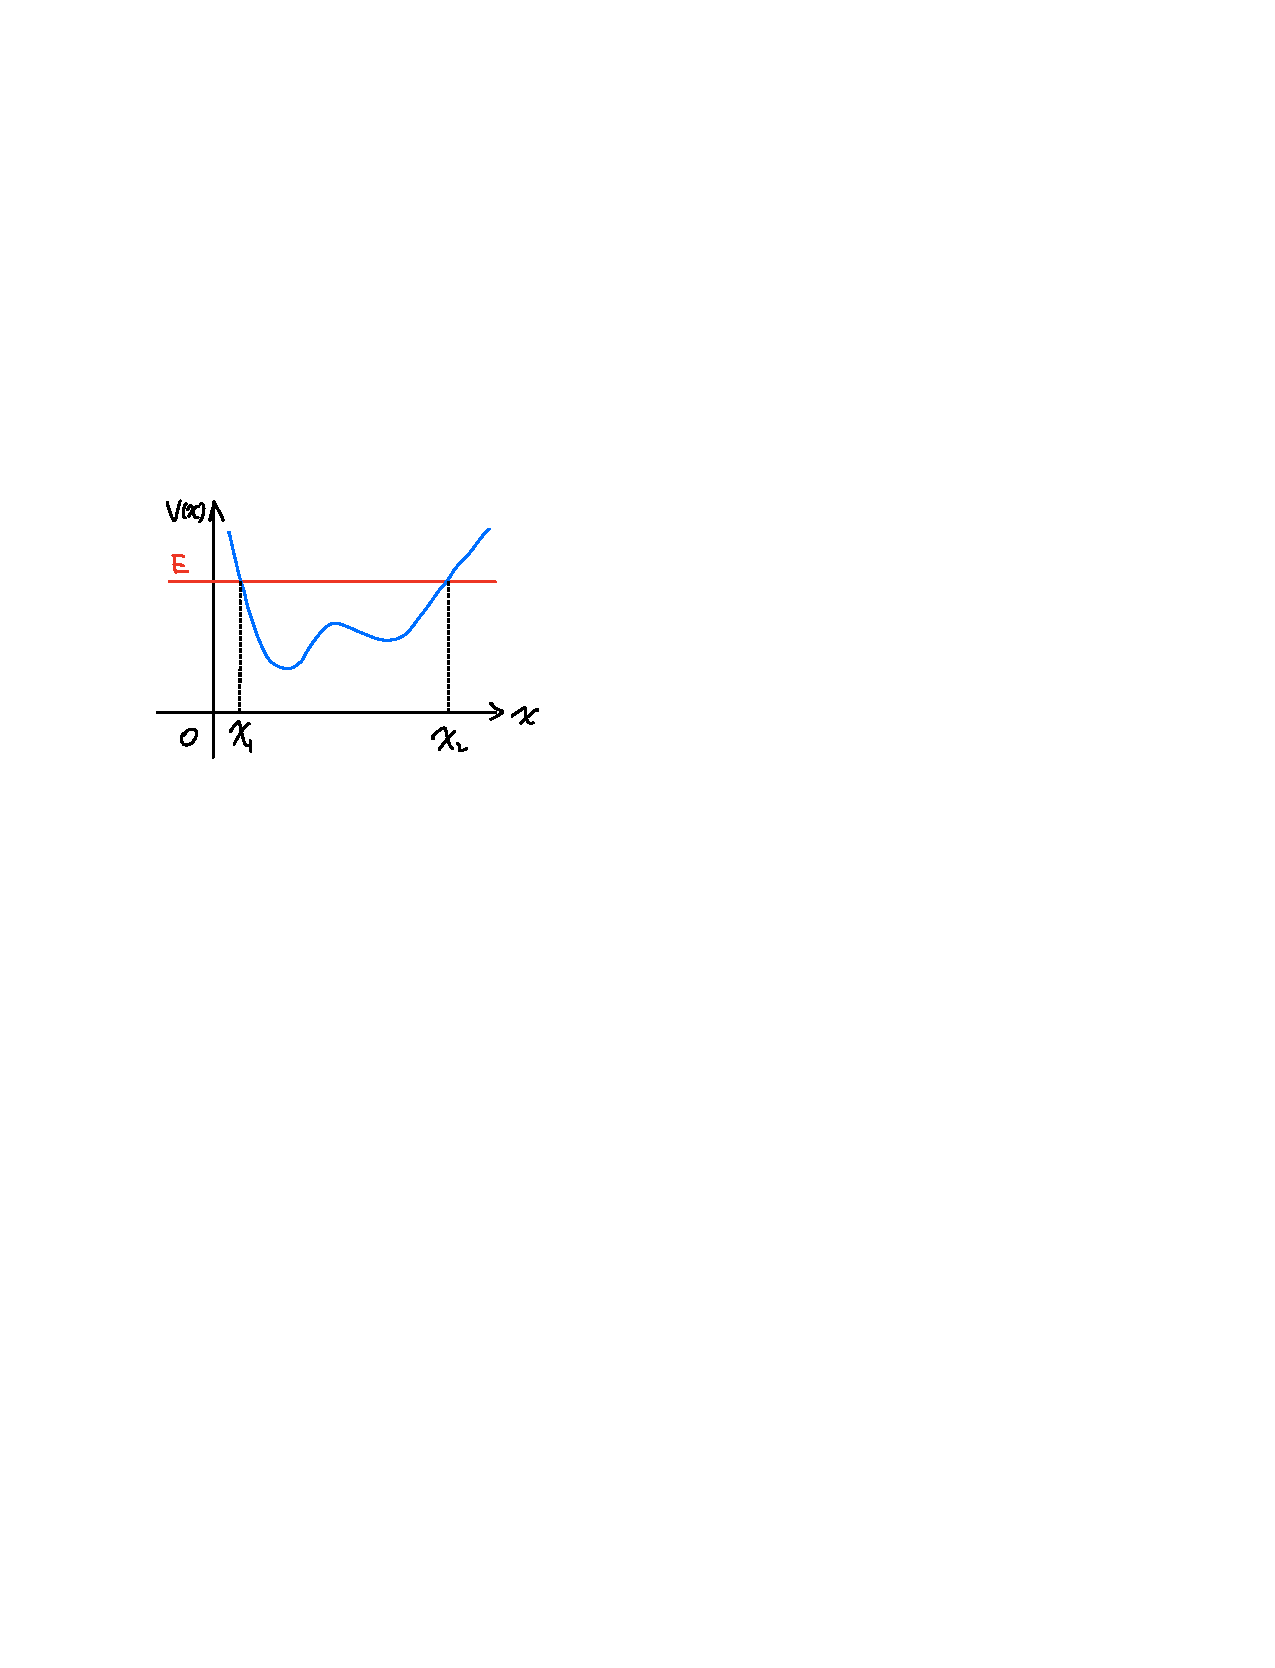
\includegraphics[width=5cm]{fig/9-1.pdf}
	\caption{WKB近似}
	\label{fig:9.1}
\end{figure}
我们首先考虑$E>V(x)$区域内WKB近似方法的基本原理,也就是图\ref{fig:9.1}中的$(x_1,x_2)$。

这一区域内定义:
\begin{equation}
	p(x)\equiv\sqrt{2m\left[E-V(x)\right]}
\end{equation}
那么定态薛定谔方程\ref{time-independent-equation}就可以改写为:
\begin{equation}
	\label{eq:9.2}
	\frac{d^2\psi}{dx^2}=-\frac{p^2}{\hbar^2}\psi(x)
\end{equation}
我们知道$\psi(x)$是个波函数,所以无非有两大要素,一是复振幅,另外是相位,所以我们可以一般的将其设为:
\[\psi(x)=A(x)\mathrm{e}^{\mathrm{i}\phi(x)}\]
代入\ref{eq:9.2}后得到两个方程:
\begin{equation}
	\label{eq:9.3}
	\begin{aligned}
		& A^{\prime\prime}-A\phi^2+\frac{p^2}{\hbar^2}A=0\\
		& A\phi^{\prime\prime}+2A^\prime\phi^\prime=0\Leftrightarrow \left(A^2\phi^\prime\right)^\prime=0
	\end{aligned}
\end{equation}

到现在为止,我们还没有进行任何近似,只是把\ref{eq:9.2}改写为了与之等价的两个方程。\ref{eq:9.3}中的第二个方程很好求解,$A^2\phi^\prime=C$,但是第一个方程
的求解难度和\ref{eq:9.2}差不多。现在我们假设$A(x)$是关于$x$的缓变函数,所以我们可以略去$A^{\prime\prime}$得到:
\[\phi^\prime(x)=\pm\frac{p}{\hbar}\Rightarrow\phi(x)=\pm\int\frac{p}{\hbar}dx\]

这个近似什么时候是合理的呢?我们知道如果$V(x)$是常数,那么最终的解为$\psi(x)\sim Ae^{ikx}$,前面的振幅是不随$x$变化的常数。这是一个正弦波,波长为$\frac{2\pi}{k}$,
只要$V(x)$在一个波长的范围内变化不大,那我们就可以认为$V(x)$近似为常函数,可见波长越小,在一个波长内$V(x)$的变化相对而言就越小,近似就越精确。而$\lambda\propto\frac{1}{k}\propto\frac{1}{\sqrt{E}}$,所以WKB近似对于高能级情况比较适用,也就是$n$很大的情况,
这时粒子的量子效应比较小。

那显然我们可以得到WKB近似下的定态波函数\footnote{$\phi(x)$中的积分因子合并到$C$中去了。}:
\begin{equation}
	\boxed{\psi(x)\approx\frac{C}{\sqrt{p(x)}}\mathrm{e}^{\pm\frac{\mathrm{i}}{\hbar}\int p(x)dx}\quad E>V(x)}
\end{equation}
所以在经典区域,我们的波函数就可以设为:
\begin{equation}
	\label{eq:9.5}
	\psi(x)\approx\frac{C_+}{\sqrt{p(x)}}\mathrm{e}^{\frac{\mathrm{i}}{\hbar}\int p(x)dx}+\frac{C_-}{\sqrt{p(x)}}\mathrm{e}^{-\frac{\mathrm{i}}{\hbar}\int p(x)dx}
\end{equation}


不过WKB近似的有效范围不能靠拐点$x_1,x_2$太近,因为显然$p(x_1)=p(x_2)=0$,上面的结果时发散的,我们后面会专门处理这种情况。
\begin{figure}[h]
	\centering
	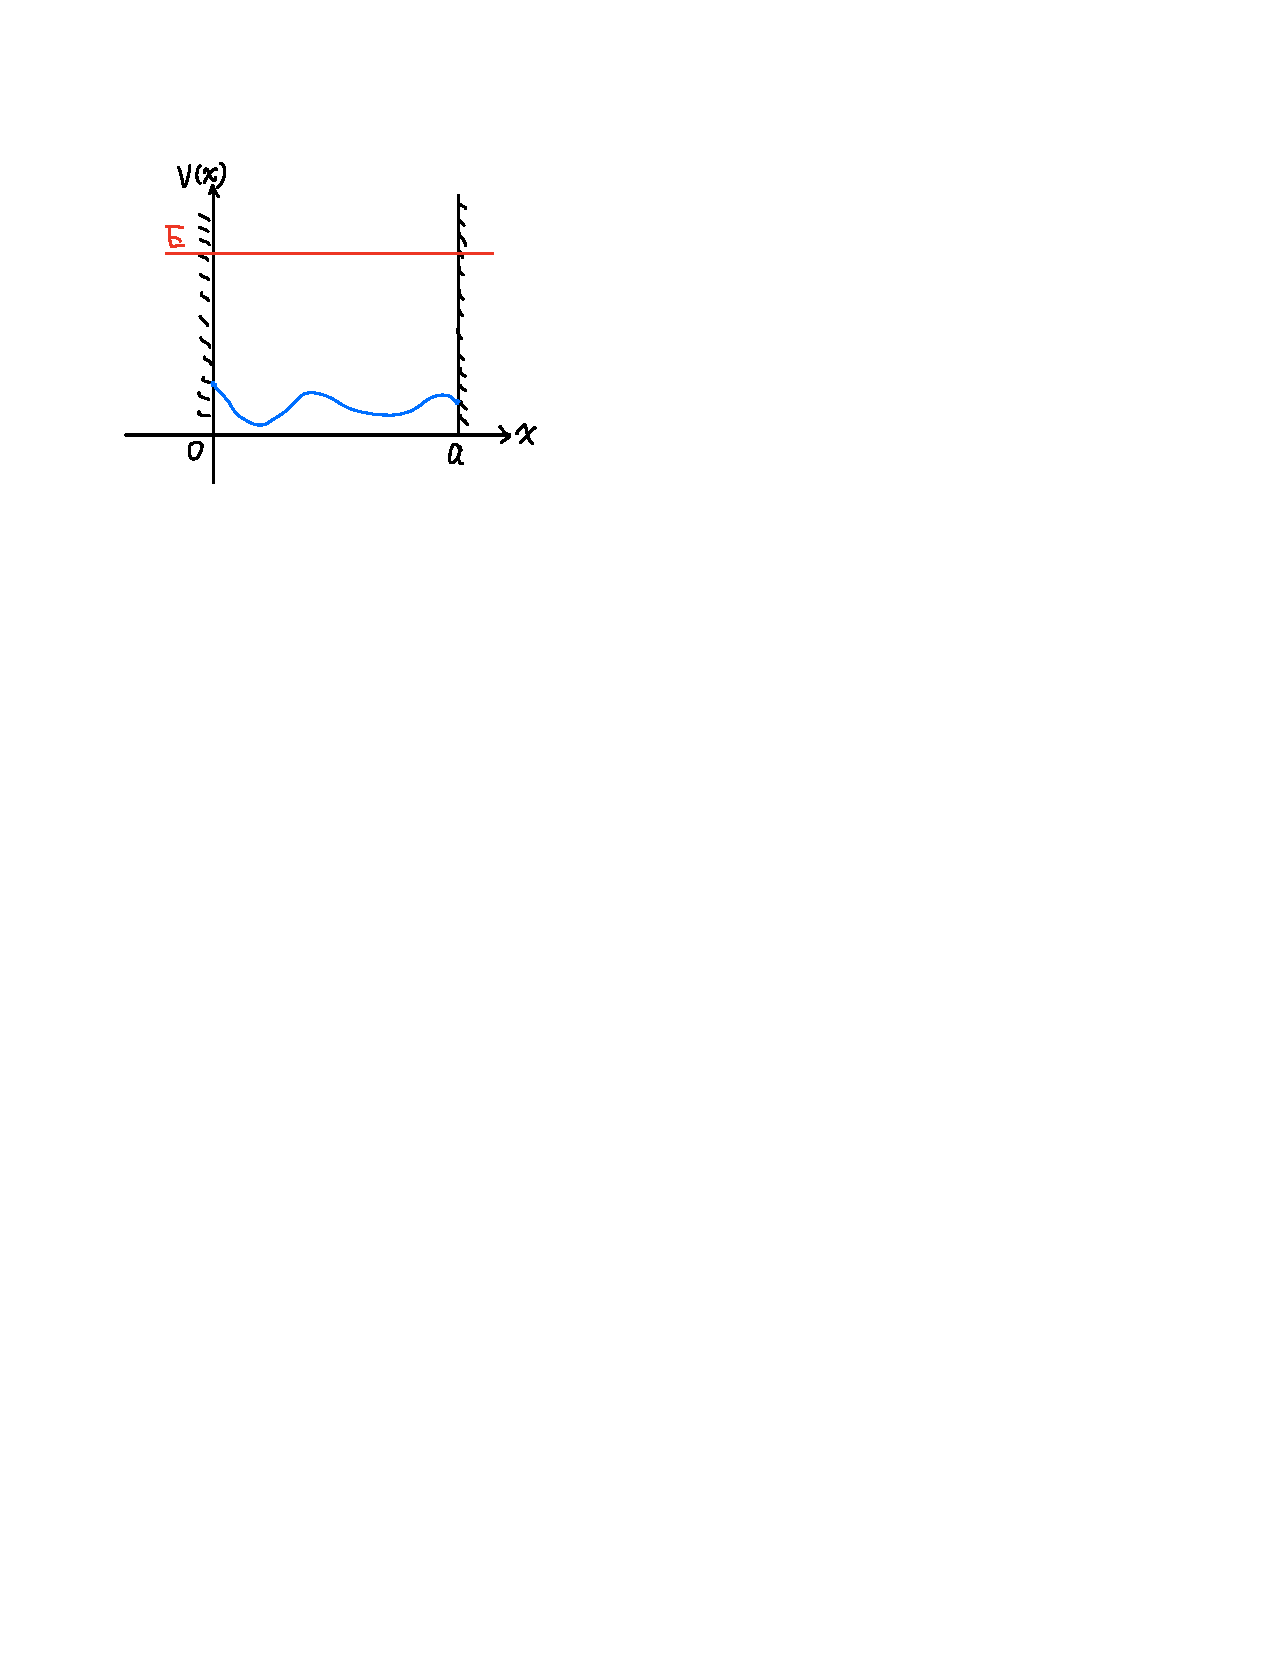
\includegraphics[width=5cm]{fig/9-2.pdf}
	\caption{两边无限高势阱}
	\label{fig:9.2}
\end{figure}
\begin{example}{两边无限高一维势阱}
	我们考虑两边无限高但是底部不一定“平坦”的势阱,之前讨论过的无限深势阱就是底部平坦$V(x)=0$的特殊情况。不过我们求解的情况是$E>V(x)$,如图\ref{fig:9.2}所示:
	
	首先我们按照\ref{eq:9.5}设波函数为:
	\[\psi(x)\approx\frac{1}{\sqrt{p(x)}}\left[C_+\mathrm{e}^{i\phi(x)}+C_-\mathrm{e}^{-i\phi(x)}\right],\quad \phi(x)=\frac{1}{\hbar}\int_{0}^{x}p(x^\prime)dx^\prime\]
	或者用三角形式:
	\[\psi(x)\approx\frac{1}{\sqrt{p(x)}}\left[C_1\sin\phi(x)+C_2\cos\phi(x)\right]\]
	然后因为势阱外部$\psi(x)=0$,所以$\psi(0)=\psi(a)=0$,所以有$C_2=0,\phi(a)=n\pi$,即:
	\begin{equation}
		\label{eq:9.6}
		\boxed{\int_{0}^{a}p(x)dx=n\pi\hbar,\quad \left(n=1,2,3,\ldots\right)}
	\end{equation}
	代入具体的$p(x)$便可以近似得出束缚态能级,而且$n$越大近似越好。对于$V(x)=0$的情况,恰好得到的就是精确解。
\end{example}
\subsection*{非经典区域}
$E<V(x)$时推导过程和前面是一样的,只是$p(x)$为纯虚数,所以近似变为:
\begin{equation}
	\boxed{\psi(x)\approx\frac{C}{\sqrt{|p(x)|}}\mathrm{e}^{\pm\frac{1}{\hbar}\int |p(x)|dx}\quad E>V(x)}
\end{equation}
\section{量子隧穿}
我们考虑的量子隧穿是两边无限高的势垒情形,这样WKB近似在拐点处就是可行的,后面我们再来考虑一般情形。
\begin{figure}[h]
	\centering
	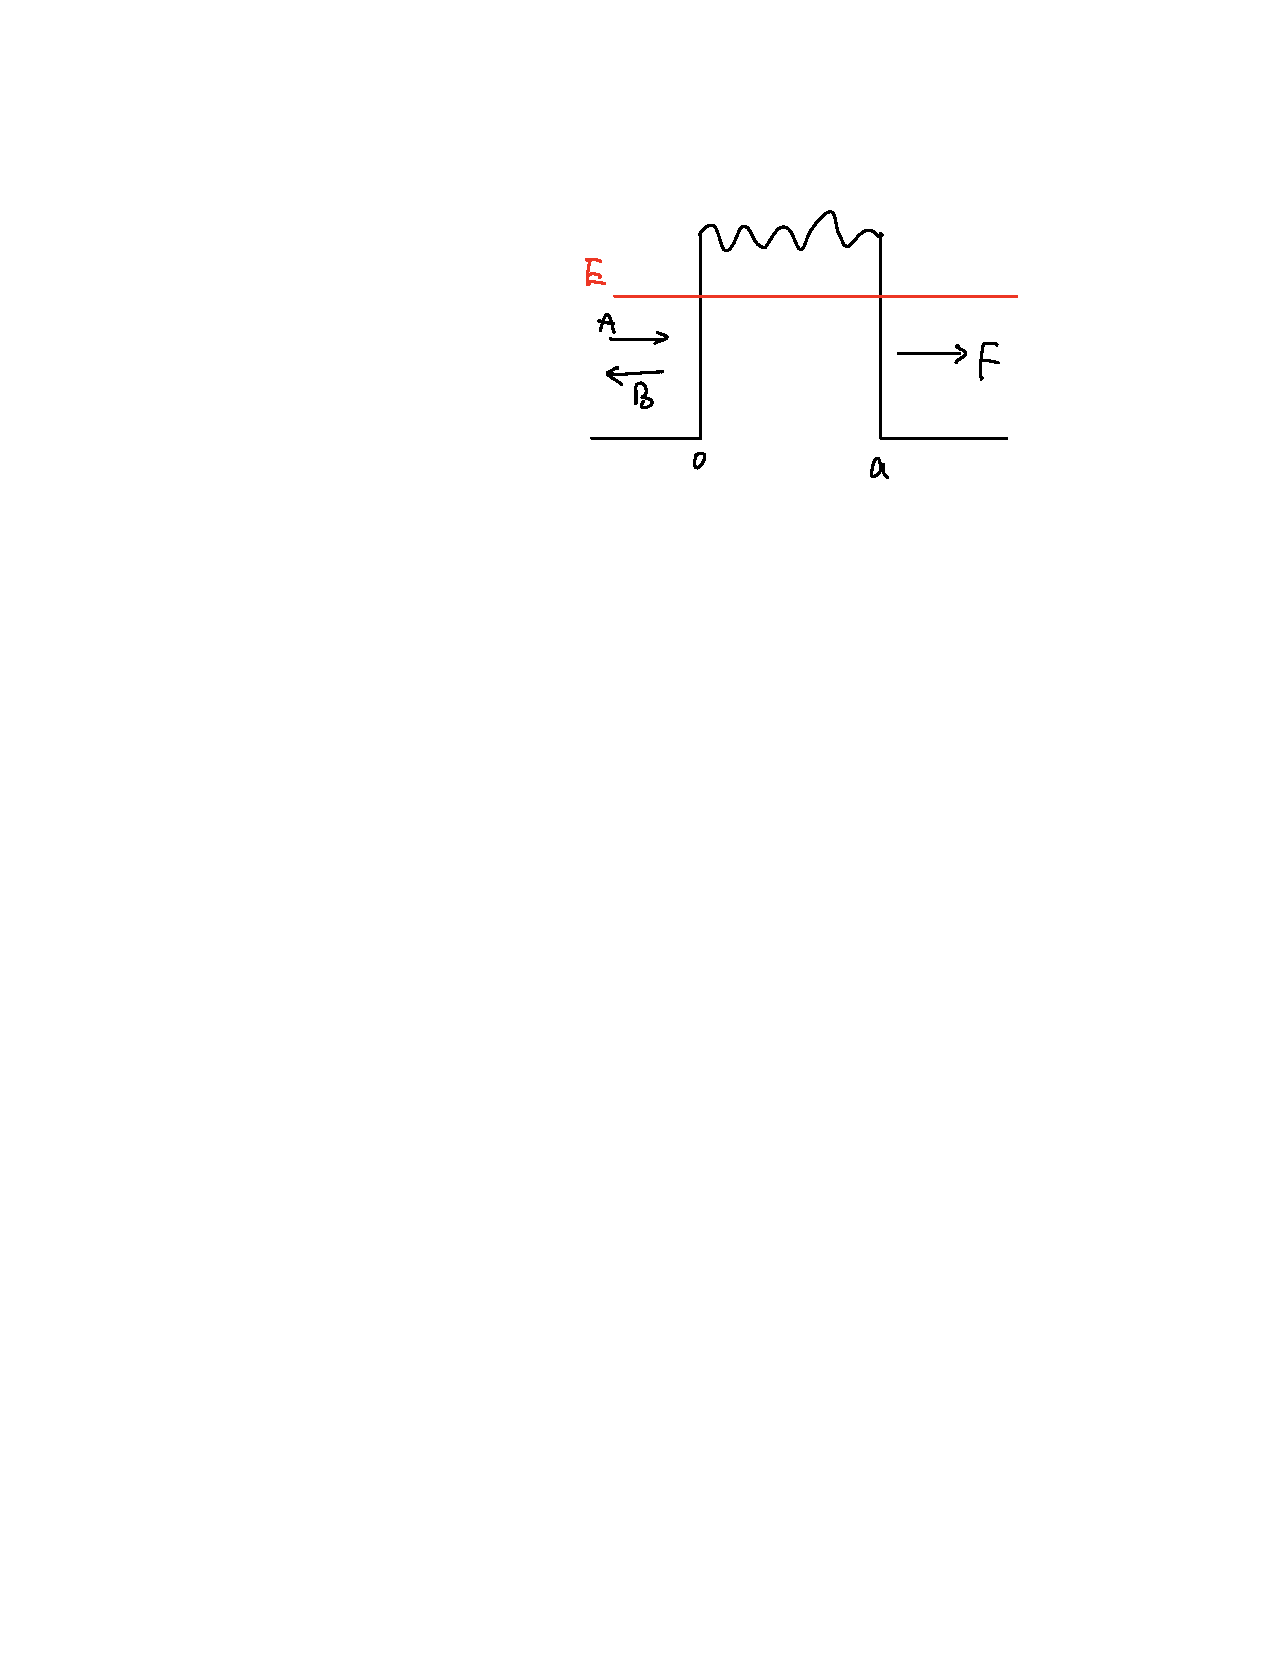
\includegraphics[width=5cm]{fig/9-3.pdf}
	\caption{量子隧穿效应}
	\label{fig:9.3}
\end{figure}
根据$\S 2.5$中对散射问题的讨论,$-\infty\to 0$有一个入射波和反射波,$a\to\infty$有一个透射波,中间是非经典区域,所以总的来说波函数可以设为:
\begin{equation}
	\psi(x)\approx\begin{cases}
		A\mathrm{e}^{ikx}+B\mathrm{e}^{-ikx}&(-\infty,0)\\
		\frac{C_+}{\sqrt{|p(x)|}}\mathrm{e}^{\pm\frac{1}{\hbar}\int |p(x)|dx}+\frac{C_-}{\sqrt{|p(x)|}}\mathrm{e}^{-\frac{1}{\hbar}\int |p(x)|dx}& (0,a)\\
		F\mathrm{e}^{ikx}&(a,+\infty)
	\end{cases}
\end{equation}
可以发现$C_+$那一项是增加透过率的,$C_-$那一项是减少透过率的。现在我们考虑\textbf{势垒很高,很厚,所以透过率很低$T\ll 1$},这样的话便可以认为$C_+\approx 0$:
\[\frac{|F|}{|A|}\sim \mathrm{e}^{-\gamma},\quad\gamma\equiv\frac{1}{\hbar}\int_{0}^{a}|p(x)|dx\]
即:
\begin{equation}
	\label{eq:9.9}
	\boxed{
		T=\frac{|F|^2}{|A|^2}\approx \mathrm{e}^{-2\gamma},\quad\gamma\equiv\frac{1}{\hbar}\int_{0}^{a}|p(x)|dx
	}
\end{equation}

\begin{figure}[h]
	\centering
	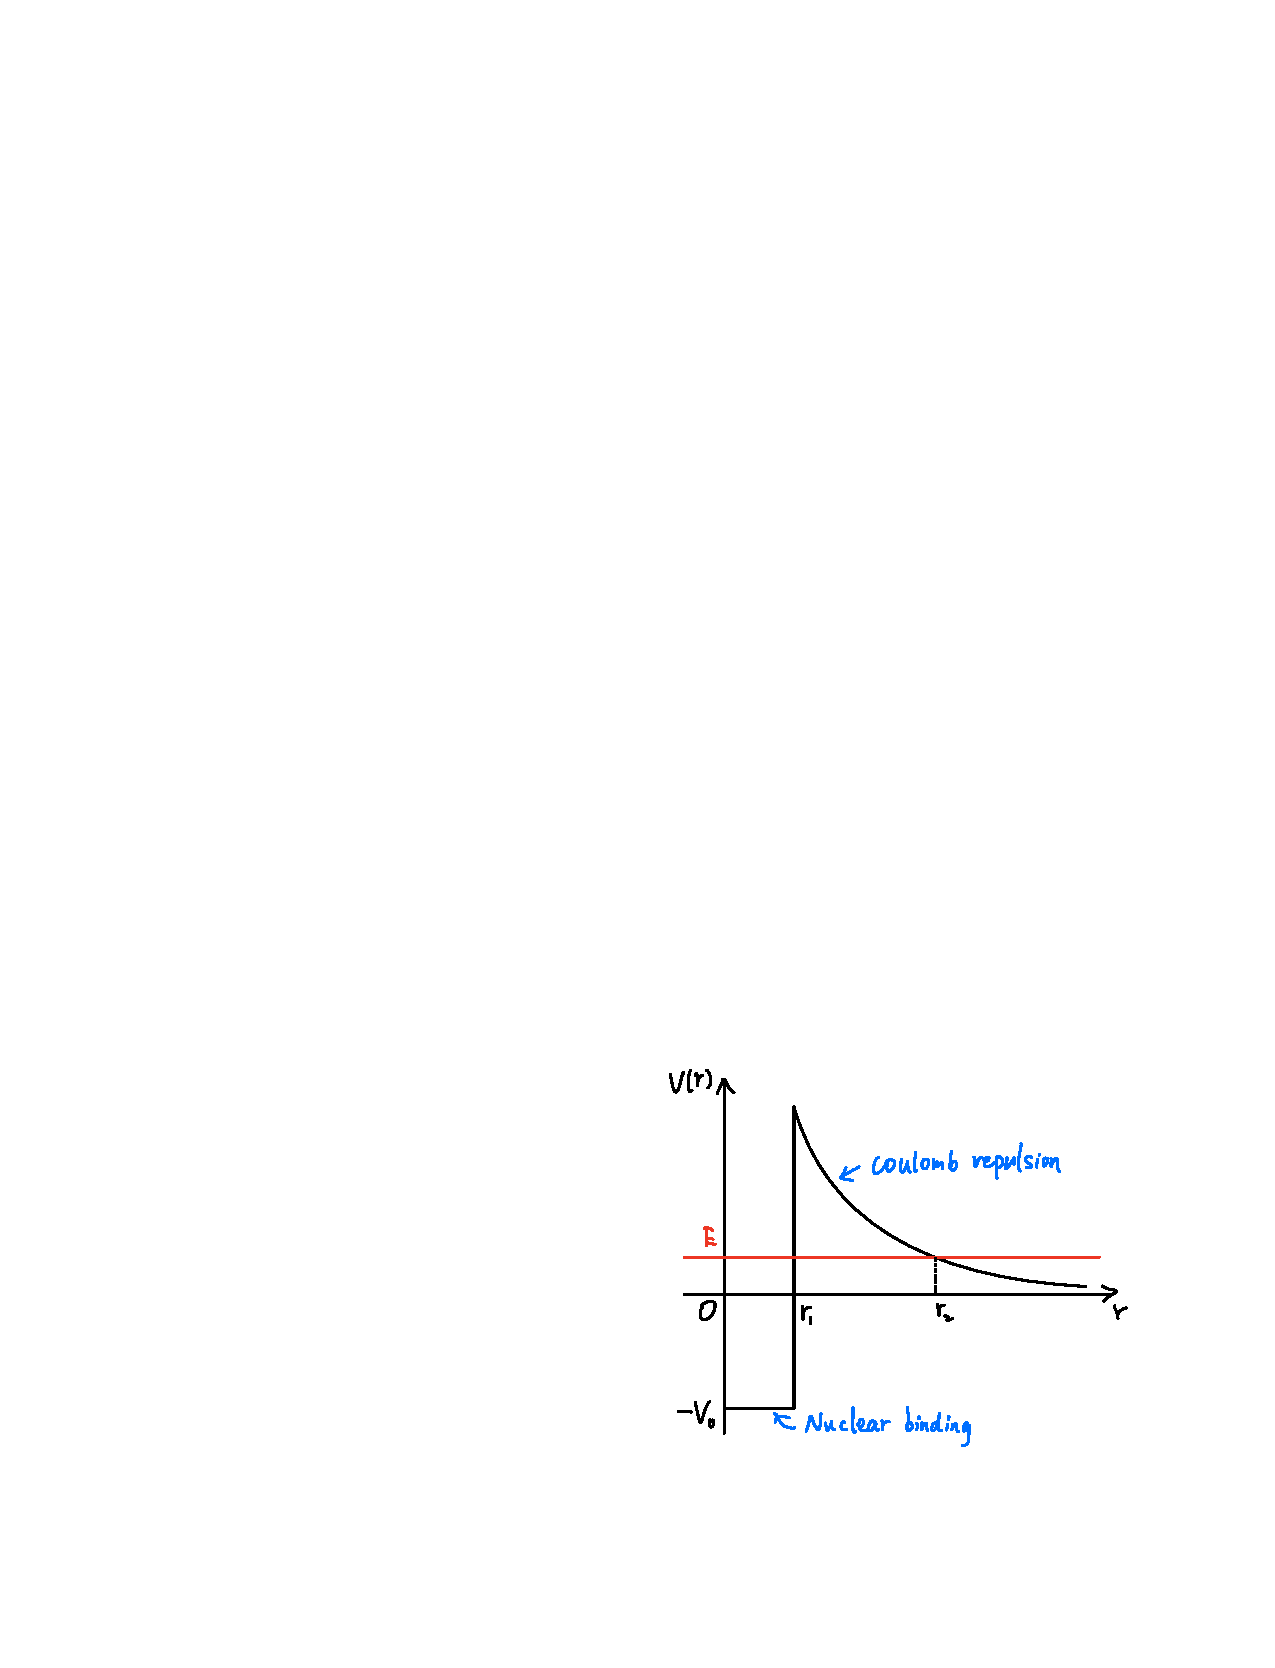
\includegraphics[width=6.5cm]{fig/9-x.pdf}
	\label{fig:9.x}
	\caption{$\alpha $衰变势垒示意图}
\end{figure}

\begin{example}{Gamow的$\alpha$衰变理论}
	所谓的$\alpha$粒子其实就是氦核$\mathrm{He}_{2}^{4}$,$\alpha$衰变就是释放$\alpha$粒子的过程。上面的理论其实可以用于近似计算$\alpha$衰变的半衰期。
	
	\setlength\parindent{2em}$\alpha$粒子带电$2e$,原子核带电$Ze$,$\alpha$粒子衰变的过程其实就是$\alpha$粒子隧穿效应离开的过程,这个势垒是一个库伦势,
	但是显然库伦势在$r=0$处发散,所以实际上我们这里的$V(r)$在$r=0$附近用一个有限深势阱来代替,$r_1$是原子核的半径。\footnote{这个问题实际上是个三维问题,不过由于各向同性而且我们是近似计算,所以丢掉离心势后考虑径向看成一维问题也没多大毛病。当然, 例如对于氢原子, 更精确的方式是根据\ref{eq:4.13}考虑离心势后进行计算。}
	其物理意义就是原子核对$\alpha$粒子的禁闭,$\alpha$粒子一般情况下就老老实实呆在$0\sim r_1$的势阱内,也就是原子核内。如图\ref{fig:9.x}所示。
	
	\setlength\parindent{2em}$E$的含义这里可以理解为出射的$\alpha$粒子的动能,可以根据质量亏损算出来,根据\ref{eq:9.9},我们计算一下$\gamma$:
	\begin{align*}
		\gamma&=\frac{1}{\hbar} \int_{r_1}^{r_2} \sqrt{2 m\left(\frac{1}{4 \pi \epsilon_0} \frac{2 Z e^2}{r}-E\right)} d r=\frac{\sqrt{2 m E}}{\hbar} \int_{r_1}^{r_2} \sqrt{\frac{r_2}{r}-1} d r\\
		&=\frac{\sqrt{2 m E}}{\hbar}\left[r_2\left(\frac{\pi}{2}-\sin ^{-1} \sqrt{\frac{r_1}{r_2}}\right)-\sqrt{r_1\left(r_2-r_1\right)}\right]
	\end{align*}
	实际上$r_1\ll r_2$,所以这里可以对上式进行小量近似得到:
	\[\gamma \approx \frac{\sqrt{2 m E}}{\hbar}\left[\frac{\pi}{2} r_2-2 \sqrt{r_1 r_2}\right]=K_1 \frac{Z}{\sqrt{E}}-K_2 \sqrt{Z r_1}\]
	其中\footnote{$1\mathrm{fm}=10^{-15}\mathrm{m}$}:
	\[K_1 \equiv\left(\frac{e^2}{4 \pi \epsilon_0}\right) \frac{\pi \sqrt{2 m}}{\hbar}=1.980 \mathrm{MeV}^{1 / 2},\quad K_2 \equiv\left(\frac{e^2}{4 \pi \epsilon_0}\right)^{1 / 2} \frac{4 \sqrt{m}}{\hbar}=1.485 \mathrm{fm}^{-1 / 2}\]
	
	\setlength\parindent{2em}现在假设$\alpha$粒子以$v$的平均速度在原子核内游走,那么它每过$\Delta t=2r_1/v$就会“碰壁”,到达$r=r_1$向外走,在经典理论中$r=r_1$是粒子速度为0,粒子不会突破原子
	核的封锁,但是量子理论由于隧穿的普遍存在,我们要考虑$\alpha$粒子穿过势垒。$\alpha$衰变的概率实际上还是比较小的,而且势垒符合前面的图\ref{fig:9.3}的形状,所以我们
	完全可以依靠\ref{eq:9.9}进行计算。所以每过时间$\Delta t$,就有$e^{-2\gamma}$的概率成功逃出一个$\alpha$粒子从而发生衰变。单个原子的lifetime为$\frac{2r_1}{v}e^{2\gamma}$.
	
	\setlength\parindent{2em}所以统计意义上来看$N$个原子的衰变速率为:
	\[\frac{dN}{dt}\approx\frac{\Delta N}{\Delta t}=Ne^{-2\gamma}\]
	显然半衰期为:$\tau=e^{2\gamma}\ln 2$
\end{example}
\section{连接公式}
现在我们开始考虑吧如何处理$E\approx V(x)$,也就是拐点附近的WKB近似问题,前面的步骤显然失效了。我们先处理束缚态,然后处理散射态,也就是一般的处理势垒隧穿行为。

\subsection*{束缚态}
我们首先看\ref{fig:9.1}中$x=x_2$附近的情况\footnote{这里说明一下,$V(x)$在$(x_1,x_2)$之外不再与$V=E$有交点。}。由于我们仅仅考虑$x_2$附近的一小段情况,所以这一段完全可以用直线替代曲线,也即:
\[V(x)\approx E+V^\prime(x_2)(x-x_2),\quad V^\prime(x_2)>0\]
在$x=x_2$两侧,但是却又离$x_2$没有那么近的区域可以用常规的WKB近似设$\psi(x)$为:
\begin{equation}
	\label{eq:9.10}
	\psi(x)\approx\begin{cases}
		\frac{A}{\sqrt{p(x)}}\mathrm{e}^{\frac{i}{\hbar}\int_{x_2}^{x}p(x)dx}+\frac{B}{\sqrt{p(x)}}\mathrm{e}^{-\frac{i}{\hbar}\int_{x_2}^{x}p(x)dx}&x<x_2\\
		\frac{C}{\sqrt{|p(x)|}}\mathrm{e}^{-\frac{1}{\hbar}\int_{x_2}^{x}|p(x)|dx}+\frac{D}{\sqrt{|p(x)|}}\mathrm{e}^{\frac{1}{\hbar}\int_{x_2}^{x}|p(x)|dx}&x>x_2
	\end{cases}
\end{equation}
至于前面的WKB失效的那一部分我们假设波函数为$\psi_p(x)$. 注意到$V(x)$的线性化以及令:
\begin{equation}
	\alpha\equiv\left[\frac{2m}{\hbar^2}V^\prime(x_2)\right]^\frac{1}{3}\quad z\equiv\alpha(x-x_2)
\end{equation}
那么$\psi_p(x)$的定态方程可以简化为:
\begin{equation}
	\frac{d^2\psi_p}{dz^2}=z\psi_p(z)
\end{equation}

这个方程是\textbf{艾里方程},解是特殊函数Airy function\footnote{进一步了解请前往:\url{https://en.wikipedia.org/wiki/Airy_function}}:
\[\psi_p(z)=a\mathrm{Ai}(z)+b\mathrm{Bi}(z)\]

现在我们的任务是确定$a$和$b$.主要思想就是$\psi_p(x)$起的是一个粘合剂的作用,把$x_2$两边的波函数连接起来。这个$\psi_p(x)$的区域有点微妙,既要足够宽,让之外的WKB近似
不足以失效;又要足够窄,这样才能对$V(x)$进行线性化近似。

$x>x_2$附近,$|p(x)|=\hbar\alpha\sqrt{z}$,根据\ref{eq:9.10}我们得知WKB近似给出的波函数为\footnote{这里$D=0$是因为要保证$\psi(x)\to 0(x\to\infty)$.}:
\begin{equation}
	\label{eq:9.13}
	\psi(z)\approx\frac{C}{\sqrt{\alpha\hbar}z^{1/4}}\mathrm{e}^{-\frac{2}{3}z^{\frac{3}{2}}}
\end{equation}
艾里函数在$z\gg 0$时有下面的渐进行为:
\begin{eqnarray}
	\left.\begin{array}{l}
		\operatorname{Ai}(z) \sim \frac{1}{2 \sqrt{\pi} z^{1 / 4}} e^{-\frac{2}{3} z^{3 / 2}} \\
		\operatorname{Bi}(z) \sim \frac{1}{\sqrt{\pi} z^{1 / 4}} e^{\frac{2}{3} z^{3 / 2}}
	\end{array}\right\} z \gg 0
\end{eqnarray}

而$\alpha\propto\hbar^{2/3},\hbar\sim 10^{-34}$,所以我们完全可以认为在$\psi_p(x)$过渡到WKB近似良好的$x>x_2$那一段$z\gg 0$,这样我们便有:
\begin{equation}
	\label{eq:9.15}
	\psi_{p}(x) \approx \frac{a}{2 \sqrt{\pi}z^{1 / 4}} e^{-\frac{2}{3}(z^{3 / 2}}+\frac{b}{\sqrt{\pi}z^{1 / 4}} e^{\frac{2}{3}z^{3 / 2}}
\end{equation}
比较\ref{eq:9.13}和\ref{eq:9.15}得到:
\[a=2C\sqrt{\frac{\pi}{\alpha\hbar}},b=0\]

同样的方法我们再看$x<x_2$那一段,首先依据\ref{eq:9.10}以及$p(x)=\hbar\alpha\sqrt{-z}$得到:
\begin{equation}
	\label{eq:9.16}
	\psi(z)\approx\frac{A}{\sqrt{\hbar\alpha}(-z)^{1/4}}\mathrm{e}^{-i\frac{2}{3}(-z)^\frac{3}{2}}+\frac{B}{\sqrt{\hbar\alpha}(-z)^{1/4}}\mathrm{e}^{i\frac{2}{3}(-z)^\frac{3}{2}}
\end{equation}
对于$z\ll 0$的情况,我们也有艾里函数渐进形式:
\begin{equation}
	\left.\begin{array}{l}
		\operatorname{Ai}(z) \sim \frac{1}{\sqrt{\pi}(-z)^{1 / 4}} \sin \left[\frac{2}{3}(-z)^{3 / 2}+\frac{\pi}{4}\right] \\
		\operatorname{Bi}(z) \sim \frac{1}{\sqrt{\pi}(-z)^{1 / 4}} \cos \left[\frac{2}{3}(-z)^{3 / 2}+\frac{\pi}{4}\right]
	\end{array}\right\} z \ll 0
\end{equation}
注意到现在我们已经有$b=0$,所以得到:
\begin{equation}
	\label{eq:9.18}
	\psi_{p}(x) \approx \frac{a}{\sqrt{\pi}(-z)^{1 / 4}} \sin \left[\frac{2}{3}(-z)^{3 / 2}+\frac{\pi}{4}\right]
\end{equation}
利用Euler公式化三角函数为指数形式后比较\ref{eq:9.16}和\ref{eq:9.18}后有:
\[A=-\sqrt{\frac{\hbar\alpha}{\pi}}a\frac{e^{-\frac{\pi}{4}i}}{2i},B=\sqrt{\frac{\hbar\alpha}{\pi}}a\frac{e^{\frac{\pi}{4}i}}{2i}\]
再根据前面得到的$a$的等式,最终结果为:
\begin{equation}
	A=ie^{-\frac{\pi}{4}i}C,B=-ie^{\frac{\pi}{4}i}C,D=0
\end{equation}
所以现在$x_2$附近,也就是\ref{eq:9.10}升级为:
\begin{equation}
	\label{eq:9.20}
	\psi(x) \approx\left\{\begin{array}{ll}
		\frac{2 C}{\sqrt{p(x)}} \sin \left[\frac{1}{\hbar} \int_{x}^{x_{2}} p\left(x^{\prime}\right) d x^{\prime}+\frac{\pi}{4}\right], & x<x_{2} \\
		\frac{C}{\sqrt{|p(x)|}} \exp \left[-\frac{1}{\hbar} \int_{x_{2}}^{x}\left|p\left(x^{\prime}\right)\right| d x^{\prime}\right], & x>x_{2}
	\end{array}\right.
\end{equation}

对于拐点处势阱是\ref{fig:9.2}图中的"Vertical Well"的情况,直接用一般的的WKB近似就好了。对于图\ref{fig:9.1}所示情况就要考虑上面的连接公式来做WKB近似。

我们同样可以去计算$x=x_1$附近这样的拐点的连接公式,只是现在$V^\prime(x_1)<0$,最终结果为:
\begin{equation}
	\label{eq:9.21}
	\psi(x) \approx\left\{\begin{array}{ll}
		\frac{C^{\prime}}{\sqrt{|p(x)|}} \exp \left[-\frac{1}{\hbar} \int_{x}^{x_{1}}\left|p\left(x^{\prime}\right)\right| d x^{\prime}\right], & x<x_{1} \\
		\frac{2 C^{\prime}}{\sqrt{p(x)}} \sin \left[\frac{1}{\hbar} \int_{x_{1}}^{x} p\left(x^{\prime}\right) d x^{\prime}+\frac{\pi}{4}\right], & x>x_{1}
	\end{array}\right.
\end{equation}
现在我们用\ref{eq:9.20}和\ref{eq:9.21}来计算两个比较重要的例子。

\begin{figure}[h]
	\centering
	\subfigure[\label{fig:9.4.a}]{
		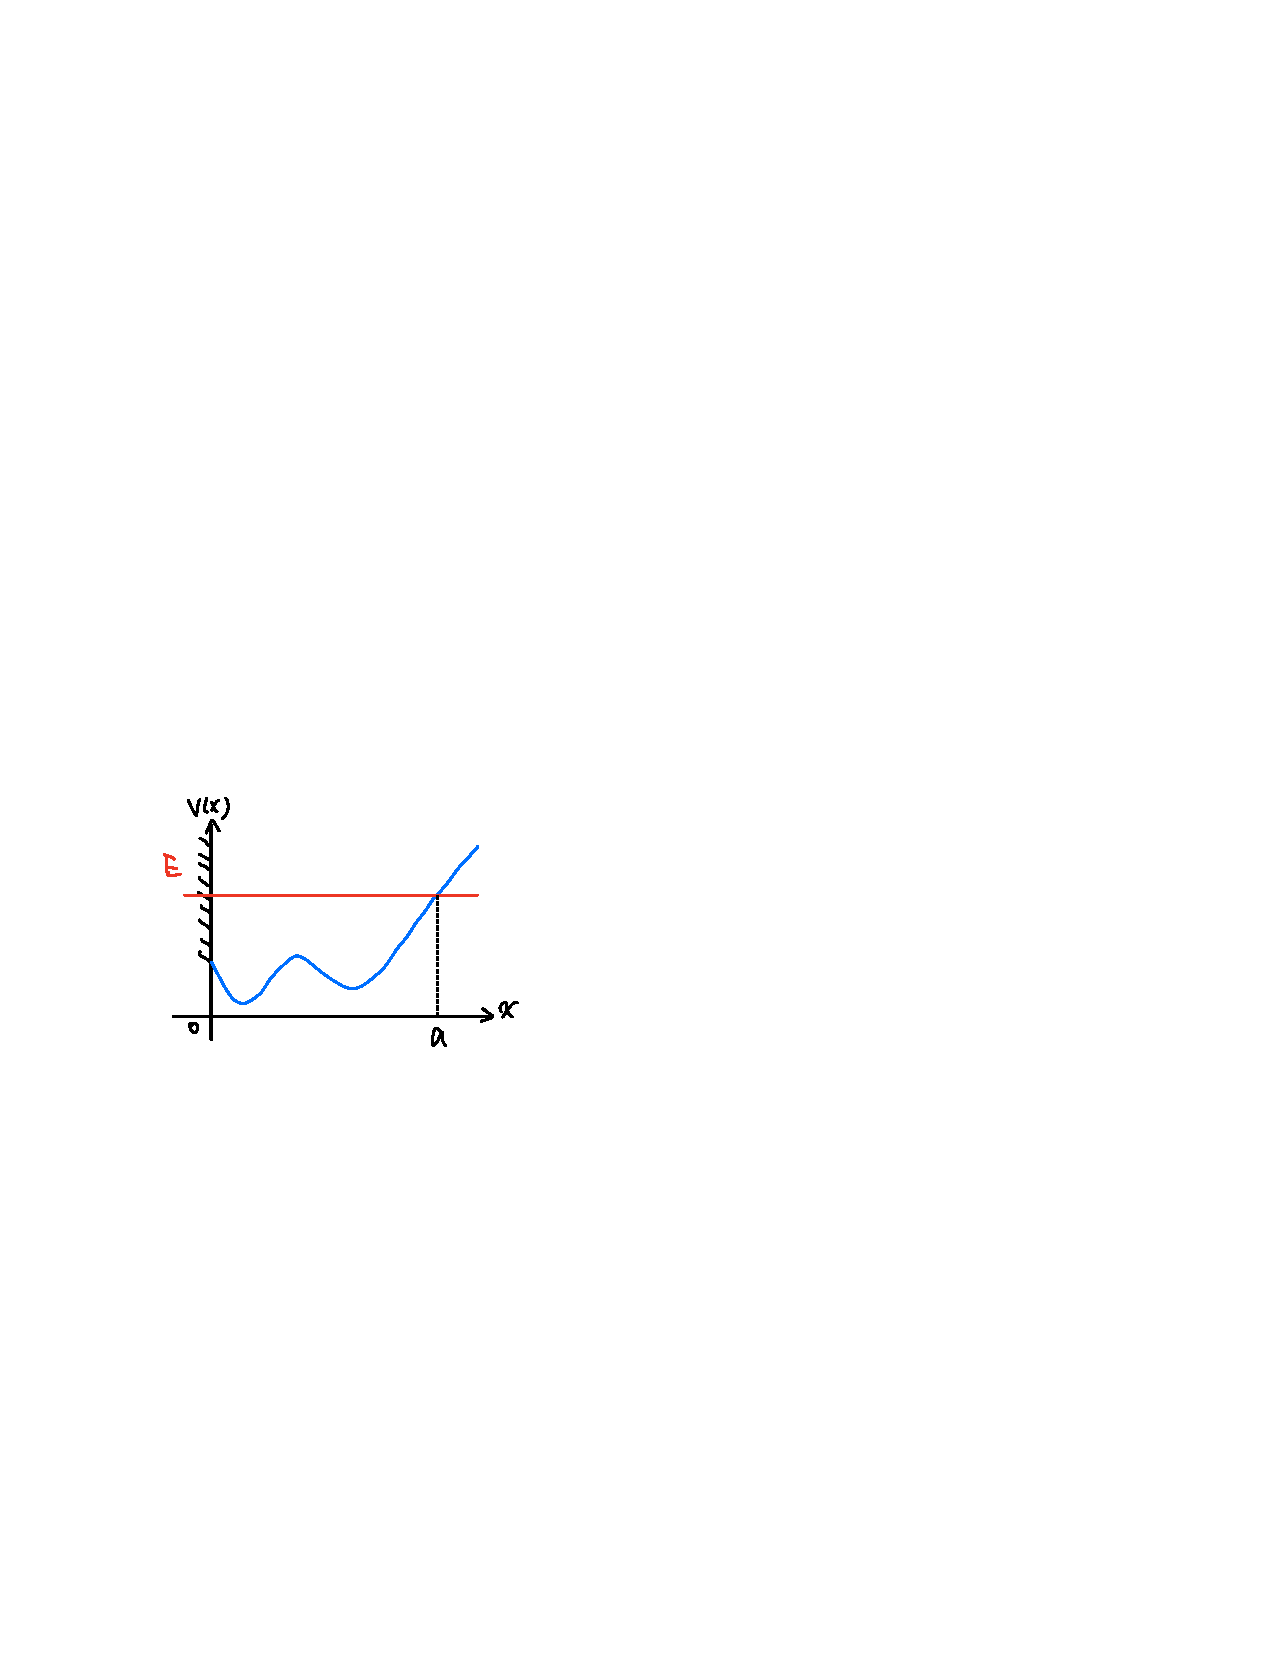
\includegraphics[width=0.45\linewidth]{fig/9-4-a.pdf}
	}\quad
	\subfigure[\label{fig:9.4.b}]{
		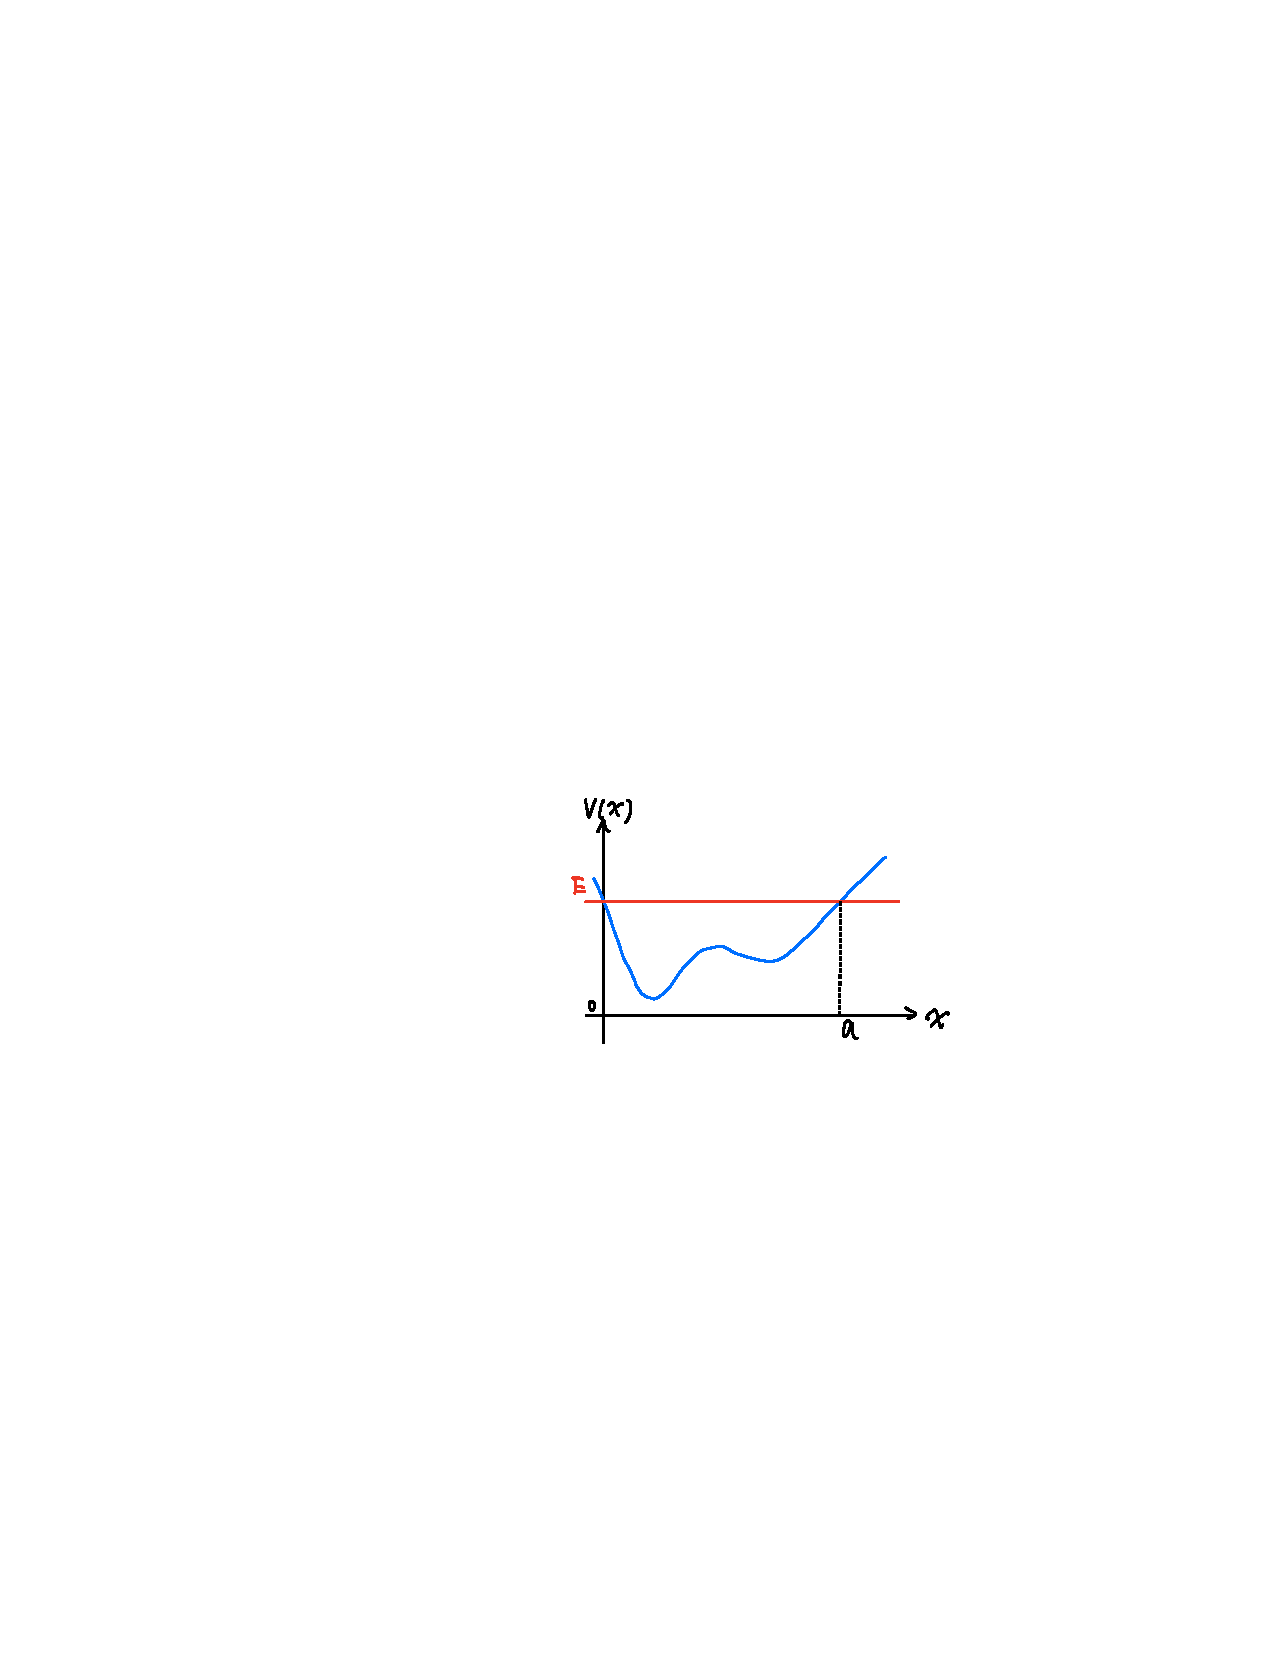
\includegraphics[width=0.45\linewidth]{fig/9-4-b.pdf}
	}
	\label{fig:9.4}
	\caption{(a)表示单边无限高势阱;(b)表示一般的势阱}
\end{figure}

\begin{example}{单边无限高一维势阱}
	现在考虑的是图\ref{fig:9.4.a}所示情况,我们只需要对$x=a$这个拐点应用连接公式。根据$\psi(0)=0$这个自然边界条件以及\ref{eq:9.20}我们得到:
	\[\frac{1}{\hbar} \int_{0}^{a} p(x) d x+\frac{\pi}{4}=n \pi, \quad(n=1,2,3, \ldots)\]
	也即:
	\begin{equation}
		\label{eq:9.22}
		\boxed{
			\int_{0}^{a} p(x) d x=\left(n-\frac{1}{4}\right) \pi \hbar
		}
	\end{equation}
	可以尝试利用这个公式解单边谐振子:
	\begin{equation*}
		V(x)=\begin{cases}
			\frac{1}{2}m\omega^2x^2&x>0\\
			\infty & x\leq 0
		\end{cases}
	\end{equation*}
	得到的是精确解
\end{example}
\begin{example}{两边都不是垂直的}
	即图\ref{fig:9.4.b}所示情况,现在我们要处理斜率为负值和正值的两类拐点。根据\ref{eq:9.20}以及\ref{eq:9.21},显然我们要求这两个式子给出的$x_1<x<x_2$区域内的$\psi(x)$是一致的,
	所以我们得到\footnote{注意这里$C$和$C^\prime$是任意的,所以我们将$D^\prime$的符号拿入$\sin$里面了}:
	\[\frac{1}{\hbar} \int_{x}^{a} p\left(x^{\prime}\right) d x^{\prime}+\frac{\pi}{4}=-\frac{1}{\hbar} \int_{0}^{x} p\left(x^{\prime}\right) d x^{\prime}-\frac{\pi}{4}+n\pi\]
	注意这里差的是$n\pi$而不是$2n\pi$正是因为$\sin$前面有任意常数$D$和$D^\prime$,化简后得到:
	\begin{equation}
		\label{eq:9.23}
		\boxed{
			\int_{0}^{a}p(x)dx=(n-\frac{1}{2})\pi\hbar,\quad(n=1,2,3,\ldots)
		}
	\end{equation}
\end{example}

我们这里导出的\ref{eq:9.22}和\ref{eq:9.23}包括前面的\ref{eq:9.6}其实是一致的,虽然看似$n$后面的常数不同,但是由于WKB近似在高能级也就是$n$很大的时候近似才愈发精确,所以后面的这些常数
实际上已经无关紧要了。

量子力学发展史上非常重要的\textbf{Bohr-Sommerfeld}量子化条件是下面的这个式子\footnote{这属于旧量子论范畴,历史上和我们这里有出入,如果读者对于量子力学的建立有兴趣可以看看{\itshape The Historical Development of Quantum Theory}这一套书。}:
\begin{equation}
	\oint pdq=\left(n-\frac{1}{2}\right)\pi\hbar
\end{equation}

如果对经典力学比较熟悉,左边实际上表示相空间轨道围成的面积,是个经典概念,右边利用普朗克常数进行量子化。在量子论发展早期这是一个及其重要的式子,当然现在
也可以用来近似计算。


\subsection*{散射态}
最后我们来考虑一下一般的散射问题,也就是现在并不是和图\ref{fig:9.3}一样的两堵墙,而考虑下图\ref{fig:9.5}所示情况:
\begin{figure}[h]
	\centering
	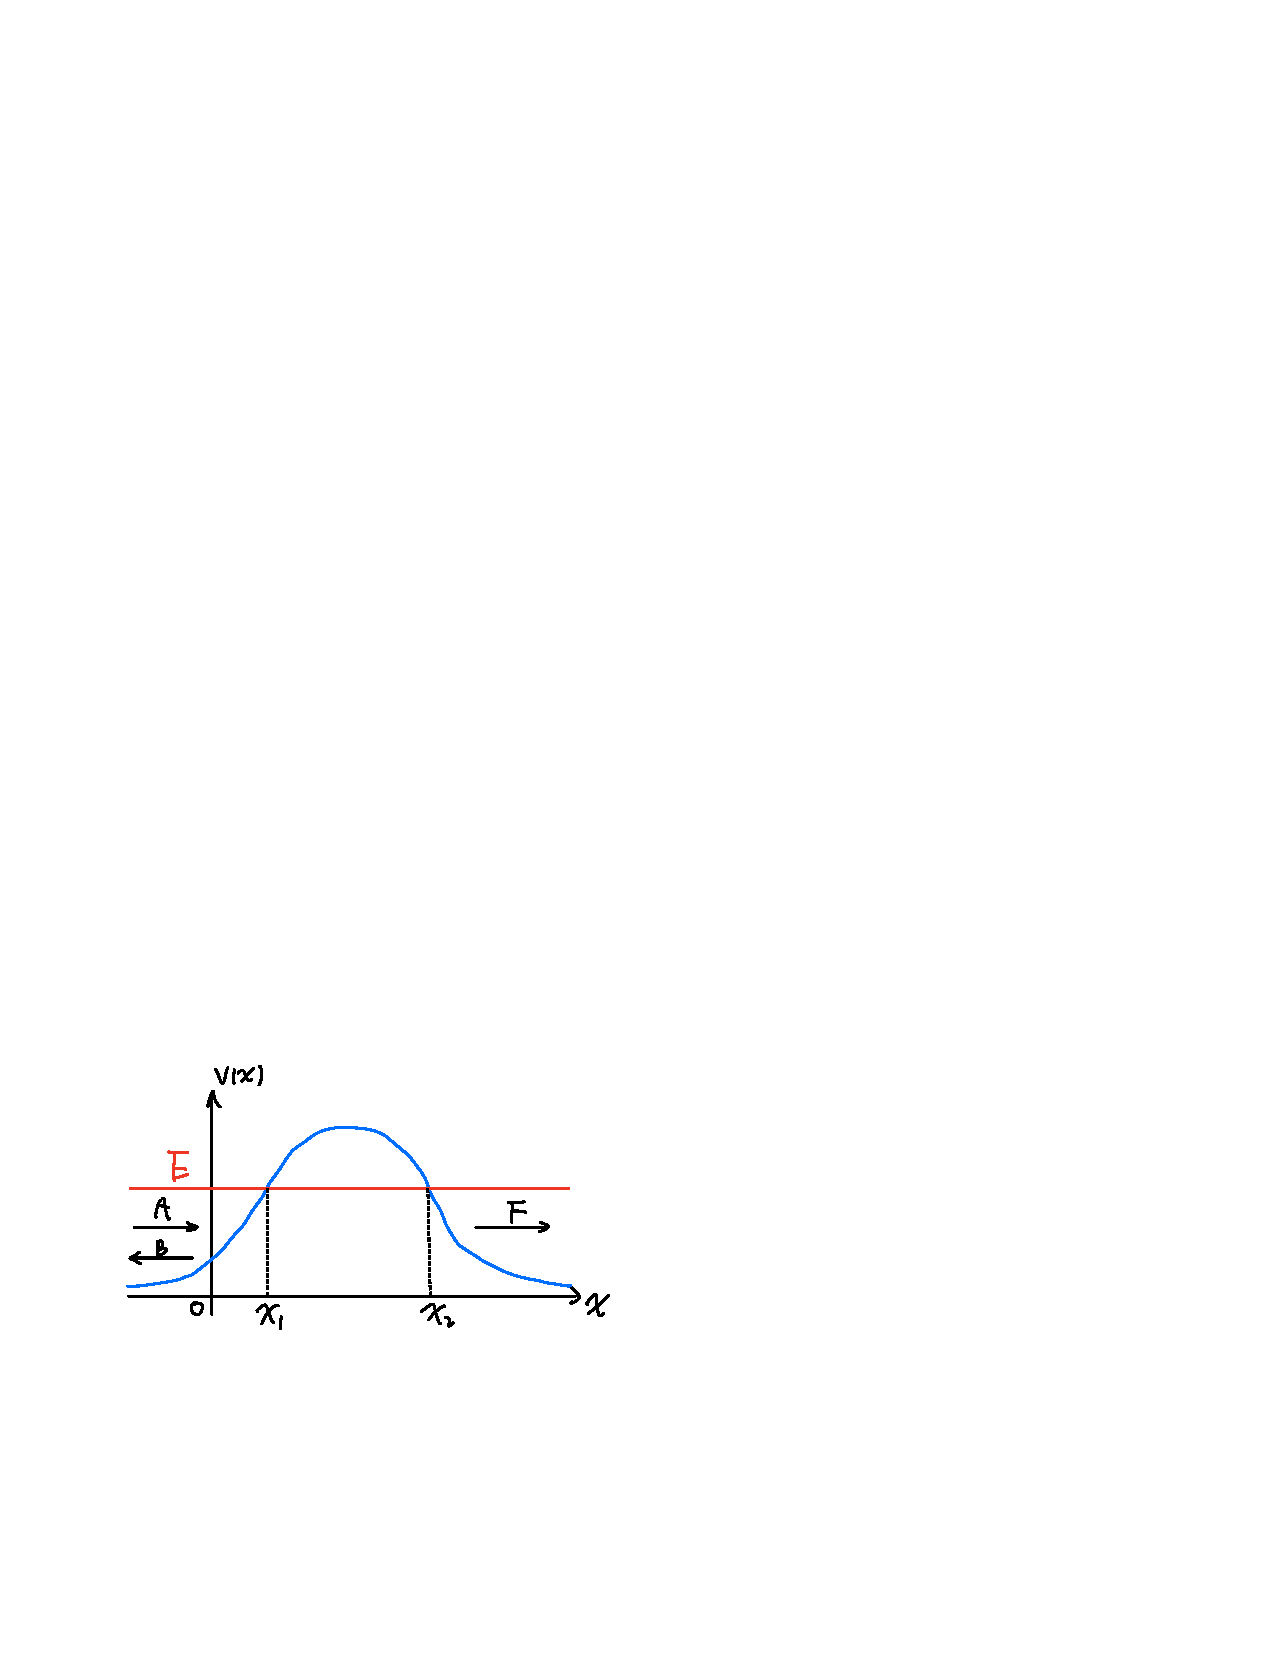
\includegraphics[width=6cm]{fig/9-5.pdf}
	\label{fig:9.5}
	\caption{一般的量子隧穿}
\end{figure}

首先根据WKB近似我们设波函数为\footnote{细细揣摩一下这里为啥$A$这一项是向右的入射波}:
\begin{equation}
	\label{eq:9.25}
	\psi(x)=\begin{cases}
		\frac{1}{\sqrt{p(x)}}\left[Ae^{-\frac{i}{\hbar}\int_{x}^{x_1}p(x)dx}+Be^{\frac{i}{\hbar}\int_{x}^{x_1}p(x)dx}\right]& x<x_1\\
		\frac{1}{\sqrt{|p(x)|}}\left[Ce^{\frac{1}{\hbar}\int_{x_1}^{x}|p(x)|dx}+De^{-\frac{1}{\hbar}\int_{x_1}^{x}|p(x)|dx}\right]& x_1<x<x_2\\
		\frac{1}{\sqrt{p(x)}}\left[Fe^{\frac{i}{\hbar}\int_{x_2}^{x}p(x)dx}\right]&x>x_2
	\end{cases}
\end{equation}
现在我们不再假设$T\ll1,C=0$,现在对两个拐点考虑前面的过程去求连接公式。

先处理$x=x_1$拐点附近的情况,这时令:
\[\alpha\equiv\left[\frac{2m}{\hbar^2}V^\prime(x_1)\right]^{\frac{1}{3}}>0,z\equiv \alpha (x-x_1)\]    
后面的计算过程和前面处理束缚态时的一样,这里就不再赘述了。
\subsubsection*{$x<x_1$}
\begin{equation}
	A=\sqrt{\frac{\hbar \alpha}{\pi}}\left(\frac{i a+b}{2}\right) e^{-i \pi / 4} , \quad B=\sqrt{\frac{\hbar \alpha}{\pi}}\left(\frac{-i a+b}{2}\right) e^{i \pi / 4}
\end{equation}
\subsubsection*{$x>x_1$}
\begin{equation}
	a=2 D \sqrt{\frac{\pi}{\alpha \hbar}}, \quad b=C \sqrt{\frac{\pi}{\alpha \hbar}}
\end{equation}
合起来即有:
\begin{equation}
	A=\left(\frac{C}{2}+i D\right) e^{-i \pi / 4} , \quad B=\left(\frac{C}{2}-i D\right) e^{i \pi / 4}
\end{equation}

然后再考虑$x=x_2$这个拐点,令:
\[\beta\equiv-\left[\frac{2m}{\hbar^2}V^\prime(x_1)\right]^{\frac{1}{3}}>0,z^\prime\equiv\beta(x-x_2)\]

前面的\ref{eq:9.25}在这里不好使了,因为它是以$x_1$为中心写的,现在我们要考虑积分限为$x_2$的情况。当然,我们大可不必重新设一个波函数再去比较系数,我们完全可以在之前的基础上改造为:
\begin{equation}
	\psi(x)\approx\frac{1}{\sqrt{|p(x)|}}\left[C e^{\frac{1}{h} \int_{x_1}^{x_2}\left|p\left(x^{\prime}\right)\right| d x^{\prime}+\frac{1}{h} \int_{x_2}^x\left|p\left(x^{\prime}\right)\right| d x^{\prime}}+D e^{-\frac{1}{h} \int_{x_1}^{x_2}\left|p\left(x^{\prime}\right)\right| d x^{\prime}-\frac{1}{h} \int_{x_2}^x\left|p\left(x^{\prime}\right)\right| d x^{\prime}}\right]
\end{equation}
令:
\[\gamma\equiv\frac{1}{\hbar}\int_{x_1}^{x_2}|p(x)|dx,C^\prime\equiv Ce^\gamma,D^\prime=De^{-\gamma}\]
则波函数可以设为我们熟悉的形式:
\begin{equation}
	\psi(x)\approx\frac{1}{\sqrt{|p(x)|}}\left[C^\prime e^{\frac{1}{\hbar}\int_{x_2}^{x}|p(x)|dx}+D^\prime e^{-\frac{1}{\hbar}\int_{x_2}^{x}|p(x)|dx}\right]
\end{equation}
连接处的波函数解为:
\[\psi_p(z^\prime)=a^\prime\mathrm{Ai}(z^\prime)+b^\prime\mathrm{Bi}(z^\prime)\]
还是前面一样的算法,不难得到:
\subsubsection*{$x<x_2$}
\begin{equation}
	a^\prime=2\sqrt{\frac{\pi}{\beta\hbar}}C^\prime,\quad b^\prime=\sqrt{\frac{\pi}{\beta\hbar}}D^\prime
\end{equation}
\subsubsection*{$x>x_2$}
\begin{equation}
	b^\prime-ia^\prime = 2\sqrt{\frac{\pi}{\beta\hbar}}Fe^{-i\frac{\pi}{4}},\quad b^\prime+ia^\prime=0
\end{equation}

上面推出的这些式子全部联合起来得到:
\begin{equation}
	F=e^{i\frac{\pi}{4}e^{-\gamma}D},\quad A=\frac{ie^{i\frac{\pi}{4}}}{2}\left(\frac{e^{-2\gamma}}{2}+2\right)
\end{equation}
故透射率:
\begin{equation}
	\label{eq:34}
	\boxed{
		T=\frac{|F|^2}{|A|^2}\approx \frac{e^{-2\gamma}}{\left[1+\left(e^{-2\gamma}/4\right)\right]^2}
	}
\end{equation}

显然,在$\gamma\gg 1$也就是$T\ll 1$时,\ref{eq:34}退化为\ref{eq:9.9}。而且对于经典极限,$\hbar\to 0$,$\gamma\to+\infty$,所以透射系数就趋近于0.

\subsection*{反射系数}
类似于前面一直在求的势垒贯穿问题,是$E<V_{\max}$的情况,我们可以考虑另一类$E>V_{\max}$的情况。在经典情形下粒子会从左侧完全越过势垒到右侧,不再返回,但是量子情形下,和隧穿效应类似,会有一个微弱的反射系数$R$。你如果尝试直接从\ref{fig:9.3}所示的情况下出发你会得到$R=0$的结论,所以我们需要更精细的利用WKB近似考虑图\ref{fig:9.7}(a)中能量为$E_>$的情况。如果直接在位置表象下计算,过程比较复杂而且物理意义并不明显\footnote{详见Landau书的$\S 52$}。下面我们将考虑一个对称的势垒$V(x)$并说明,位置空间波函数的反射实际上等价于其对应动量空间波函数的透射,并利用动量空间下的WKB近似来计算反射系数。\footnote{这一小节的内容引自文章:\DOI{https://doi.org/10.1119/1.3298428}}
\begin{figure}
	\centering
	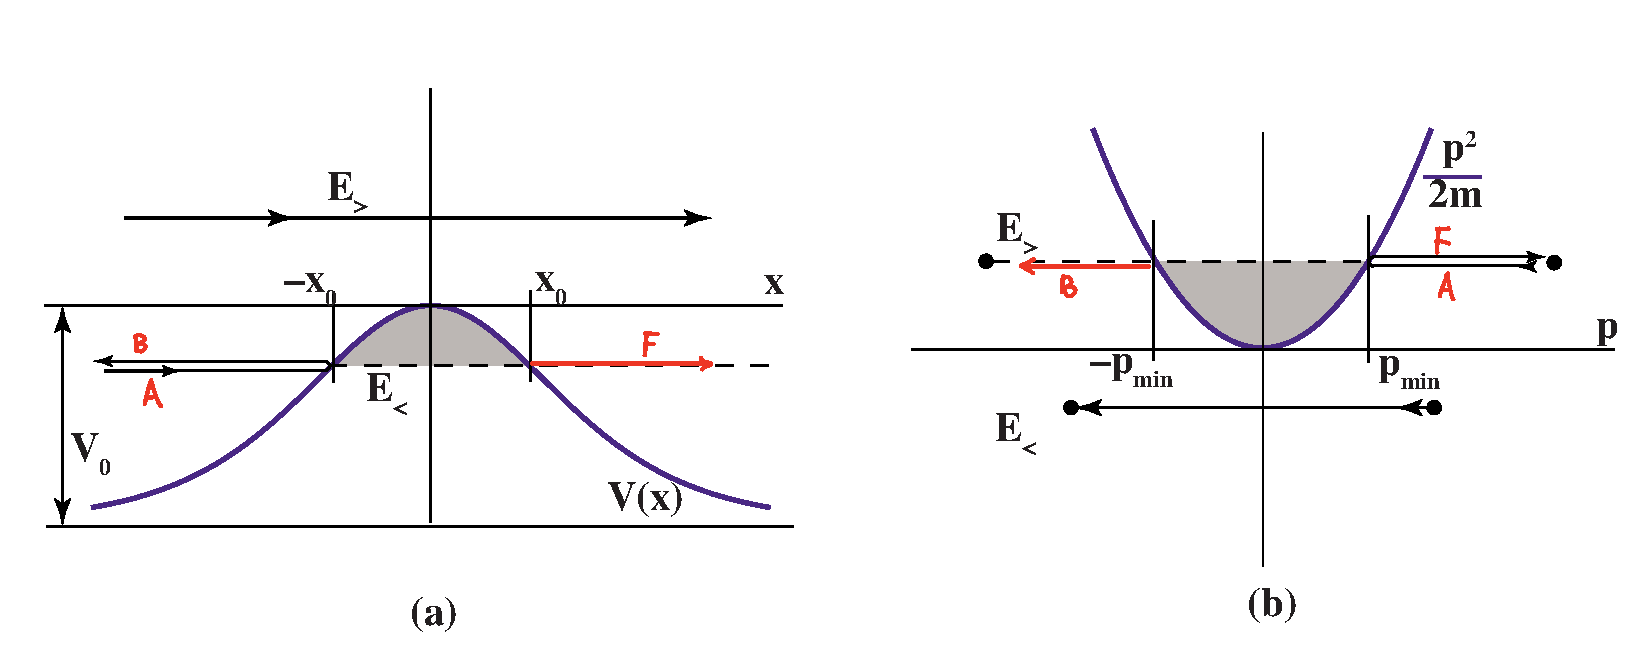
\includegraphics[width=0.8\linewidth]{fig/9-7.pdf}
	\label{fig:9.7}
	\caption{在动量空间看,位置空间中反射和透射意义互换。图a中的$A,B,F$是对$E_<$而言的,对于$E>$,箭头的端点应该放在$x=0$处。}
\end{figure}

在位置空间中左侧来的入射波复振幅为$A$,动量大于$0$而且由于$p(x)=\sqrt{2m(E-V(x))}$,所以由于$V(x)$的增大,越靠近$x=0$动量就会越小,最终达到$p_{\min}$.在动量空间看就是从右侧往左侧的入射过程,图\ref{fig:9.7}(b)中曲线是动能曲线,经典情形下在动量空间中看显然就是从右往左的入射,然后到$p=p_{\min}$后在动量空间中反射。这个反射在位置空间对应着什么呢?我们发现位置空间按中的透射波$F$正是与$A$相反动量从$p_{\min}$开始逐渐变大的一个波,所以就正好与动量空间的哪个反射波对应了。现在考虑量子效应,位置空间中还会有一个反射波$B$,它和$A$正好差了一个负号,动量从$-p_{\min}$然后随着往左走慢慢向着$-\infty$趋近,这在动量空间中看正像是穿透了阴影区域的透射波,要知道在经典力学中粒子是不可能越过阴影区域的。所以现在我们说明了在位置空间中的反射等价于动量空间中的隧穿效应。

我们下面举一个经典力学中的例子来更好的说明这一点。考虑势垒$V(x)=\frac{1}{2}m\omega^2x^2$,在相空间$p-x$中粒子的轨迹是一簇双曲线,如图\ref{fig:9.8}所示。图中$A\to B\& C\to D$在$x$上看是一种关于$p$轴透射,但是在$p$上看是关于$x$轴的反射,同理$E\to F\& H\to G$也表现你了透射和反射的角色互换。
\begin{figure}
	\centering
	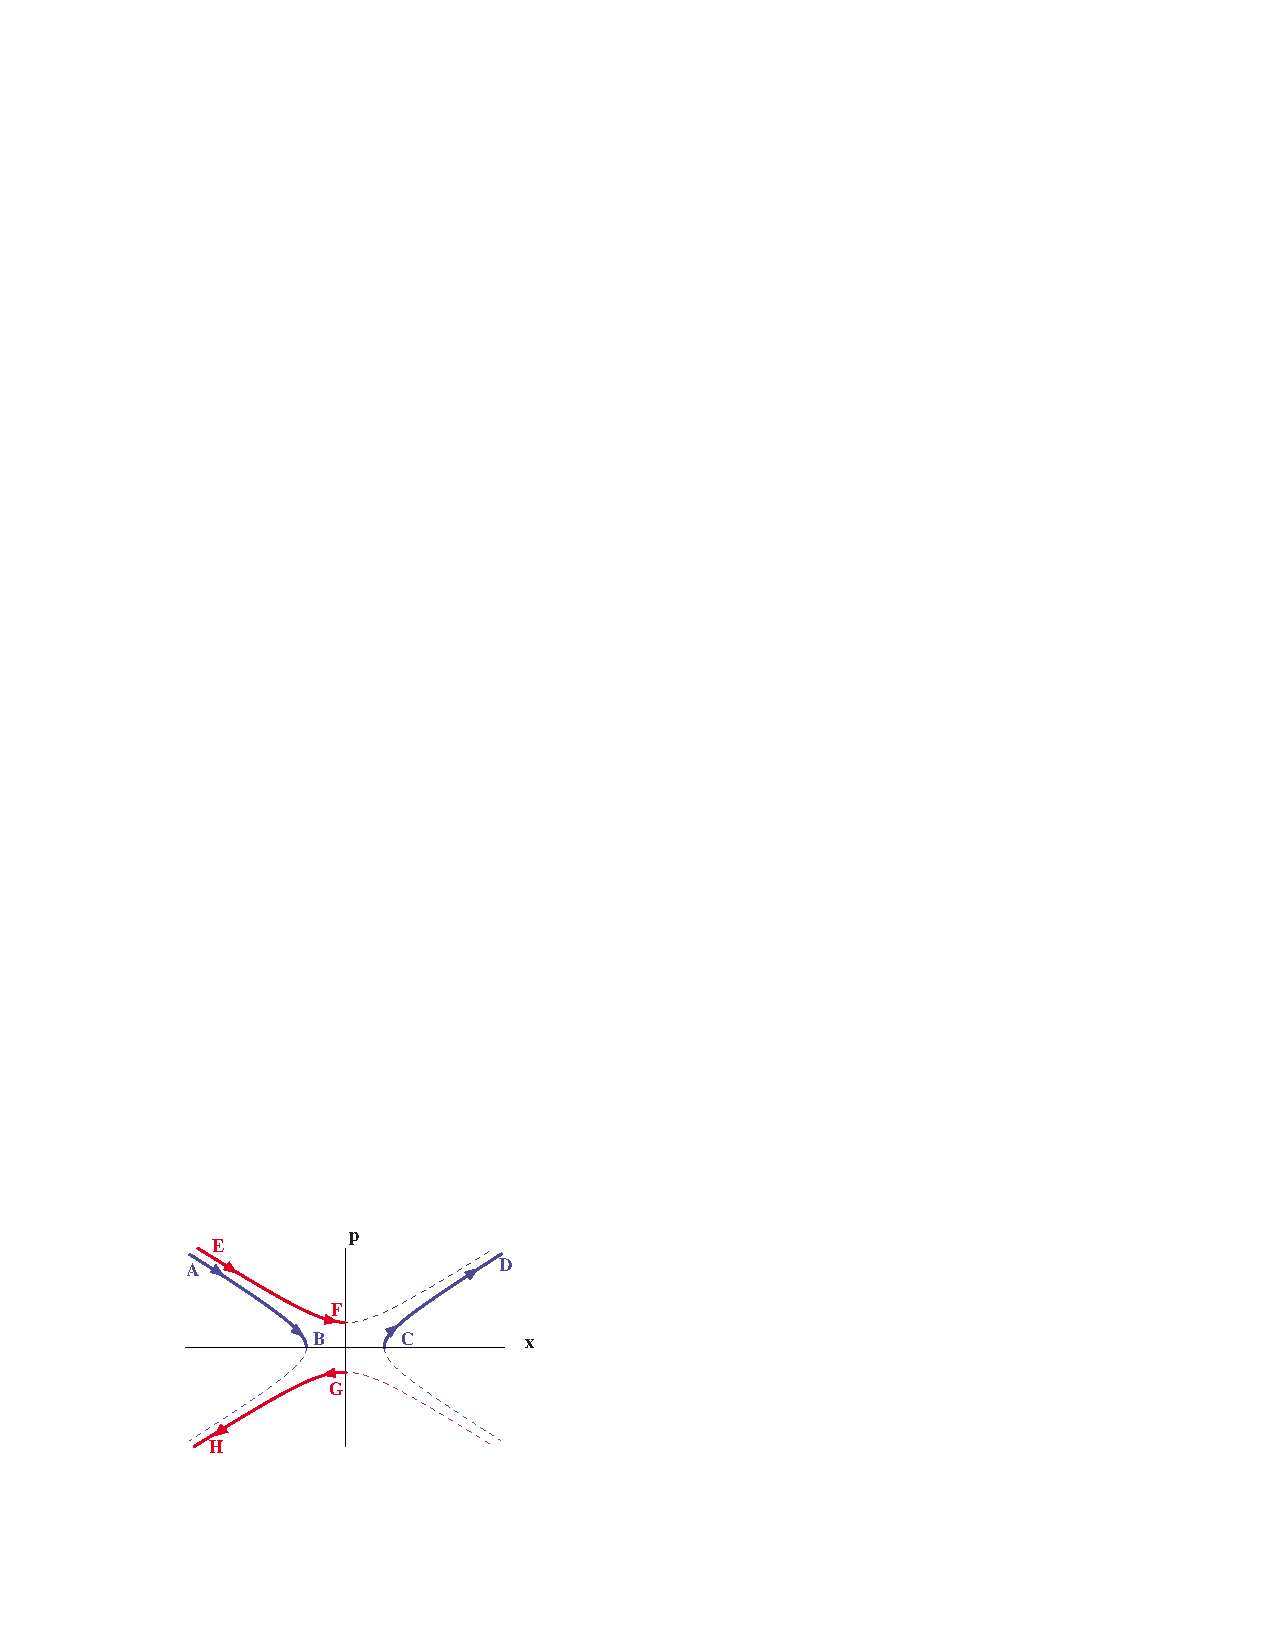
\includegraphics[width=0.65\linewidth]{fig/9-8.pdf}
	\label{fig:9.8}
	\caption{“反胡克势”下粒子相空间轨迹}
\end{figure}

现在我们在动量表象下写薛定谔定态方程,注意在动量表象下$\hat{p}\to p,\hat{x}\to i\hbar d/dp$.
\begin{equation}
	\label{eq:9.35}
	\left[\frac{p^2}{2m}+V(i\hbar\frac{d}{dp})\right]\phi(p)=E\phi(p)
\end{equation}

在动量空间下考虑WKB近似比位置空间要麻烦许多,微分算符藏在了形式未知的势能函数中。我们设动量空间波函数为:\footnote{这里并不失一般性,因为$\sigma(p)$是任意的复变函数}
\begin{equation}
	\label{eq:9.36}
	\phi(p)=e^{i\sigma(p)/\hbar}
\end{equation}

把上式带到\ref{eq:9.35}中,考虑$\sigma(p)$是缓变函数,$\sigma^{\prime\prime}(p)\approx 0$,那么我们把$V(i\hbar\frac{d}{dp})$展开幂级数,而且注意到$\sigma(p)$高阶导数近似为$0$我们得到下面的式子:
\begin{equation}
	\frac{p^2}{2m}+V(-\sigma^{\prime}(p))=E
\end{equation}
不难发现这里$-\sigma^{\prime}(p)$正是$p(x)$的反函数,我们记为$x(p)$,利用$V$的反函数$V^{-1}$可以算出:
\begin{equation}
	\sigma(p)=-\int^{p} d p^{\prime} x\left(p^{\prime}\right)=-\int^{p} d p^{\prime} V^{-1}\left(E-\frac{p^{\prime 2}}{2 m}\right)
\end{equation}

最后带入到\ref{eq:9.36}便得到了相空间中的WKB近似。这里看似只有一个解,不像位置空间中有$\pm$两个线性无关解,WKB近似设为两者的线性组合,但实际上这里是一样的,就拿反谐振子$V(x)=\frac{1}{2}\alpha x^2$来说,我们可以得到其反函数为$V^{-1}(\xi)=\pm\sqrt{2\xi/\alpha}$,也是线性无关的两个解。

考虑到$R\ll 1$,我们这里就不考虑连接公式那种情况了,类似于$\S$9.2中的考虑我们可以得到\footnote{注意在$(-p_{\min},p_{\min})$也就是经典情况不允许的区域内$x(p)$始终是纯虚数}:
\begin{equation}
	\boxed{
		R\equiv \frac{|B|^2}{|A|^2}\approx e^{-2\zeta},\quad \zeta\equiv\int_{-p_{\min}}^{p_{\min}}|x(p)|dp}
\end{equation}
或者显式写为:
\begin{equation}
	\label{eq:9.40}
	\boxed{
		R=\exp \left[-\frac{2}{\hbar} \operatorname{Im} \int_{-p_{\min }}^{p_{\min }} d p V^{-1}\left(E-\frac{p^{2}}{2 m}\right)\right]	
	}
\end{equation}
这个公式更广为人知的形式是Landau书中给出的复变函数积分形式:
\begin{equation}
	\label{eq:9.41}
	\boxed{
		R=\exp \left[-\frac{4}{\hbar} \operatorname{Im} \int_{z_{1}}^{z_{0}}  p(z)dz\right]
	}
\end{equation}

其中$p(z)=\sqrt{2m(E-V(z))}$,$z_0$是上半平面内使得$p(z_0)=0$的点。$z_1$是实轴上的任意一个点,因为$p(z)$认为是解析函数,而且$p(z)$在实轴上的取值都是实数,所以$z_1$的选取有任意性,可以根据计算的方便选取。下面我们来证明\ref{eq:9.40}和\ref{eq:9.41}等价,首先对于任意一个势垒我们都可以通过概念势能零点以及坐标原点使得$V(0)=V_{\max}=0$,然后对于对称势垒$z_0=iy_0$在虚轴上。取$z_1$沿着虚轴积分\ref{eq:9.41}得到:
\begin{align*}
	R&=\exp \left[-\frac{4}{\hbar} \operatorname{Im} \int_{0}^{y_{0}} i d y p(i y)\right]\\
	&=\exp\left[-\frac{4}{\hbar}\left(\left.y p(i y)\right|_{0} ^{y_{0}}+\int_{0}^{p_{\min }} d p y(p)\right)\right]\\
	&\overset{p(iy_0)=0}{=}\exp\left[-\frac{2}{\hbar}\int_{-p_{\min}}^{p_{\min }} d p y(p)\right]
\end{align*}
再注意到$iy(p)=V^{-1}\left(E-\frac{p^{2}}{2 m}\right)$便回归到了\ref{eq:9.40}。